\section{Exploración Espacial}\label{espacial}



Como acabamos de ver en la Tabla \ref{regresiones} en la página \pageref{regresiones}, si quisieras sintetizar la multidimensionalidad de nuestros indicadores, podr�amos usar tres de las cuatro variables que tenemos (un par de las originales tiene demasiada correlación). 

As�, propongo que calculemos conglomerados de pa�ses usando toda la información de tres de los indicadores. Como nuestras variables son ordinales utilizaremos un proceso de conglomeración donde las distancia serán calculadas usando la medida {\bf gower} propuestas en \cite{gower_general_1971}, y para los enlazamientos usaremos la técnica de {\bf medoides} según \cite{reynolds_clustering_2006}. Los tres conglomerados se muestran en la Figura \ref{clustmap}.






\begin{figure}[h]
\begin{Schunk}
\begin{Soutput}
  Group.1       IDH  cabeLog restoLog
1       1 0.8370000 14.10331 12.85966
2       2 0.7646667 13.26530 12.77460
3       3 0.7770000 10.98166 10.92973
\end{Soutput}
\end{Schunk}
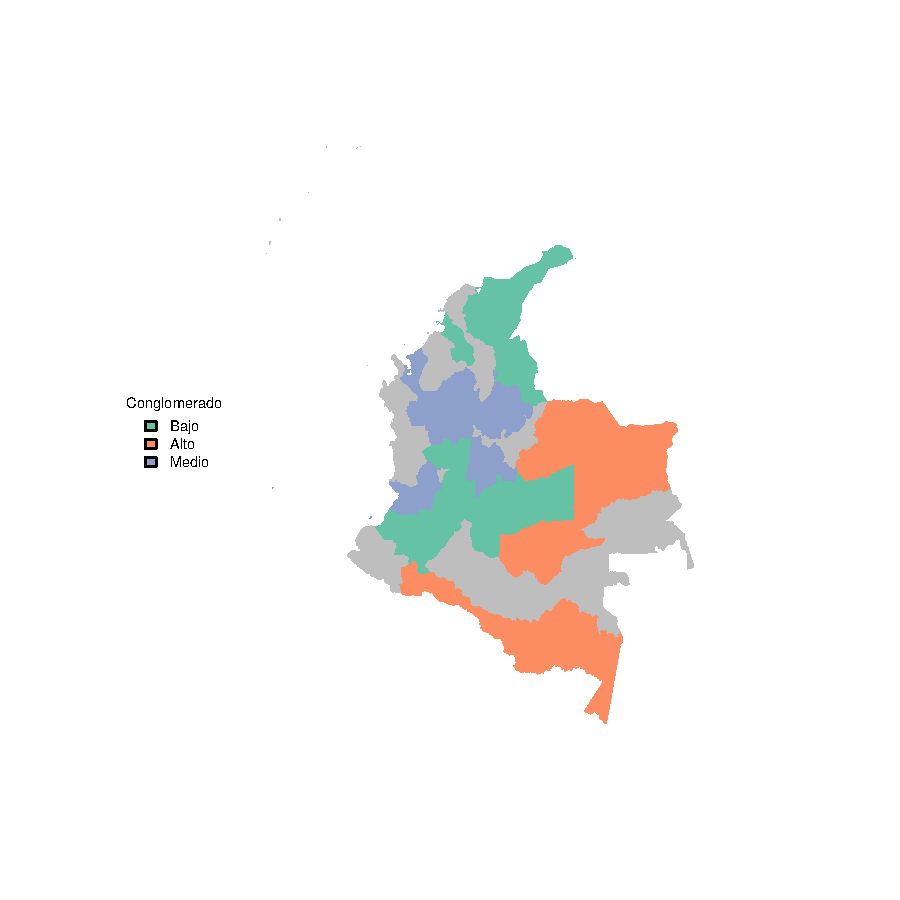
\includegraphics{espacial-plotMap1}
\caption{Paises conglomerados segun sus indicadores sociopolíticos}\label{clustmap}
\end{figure}
%%%%%%%%%%%%%%%%%%%%%%%%%%%%%%%%%%%%%%%%%%%%%%%%%%%


\endinput
